\documentclass[border=10pt]{standalone}
\usepackage[svgnames]{xcolor}
\usepackage{amsmath}
\usepackage{pgfplots}
\pgfplotsset{compat=newest}
\usepackage[sfdefault]{FiraSans}
\usepackage{FiraMono}
\renewcommand*\familydefault{\sfdefault}
\begin{document}
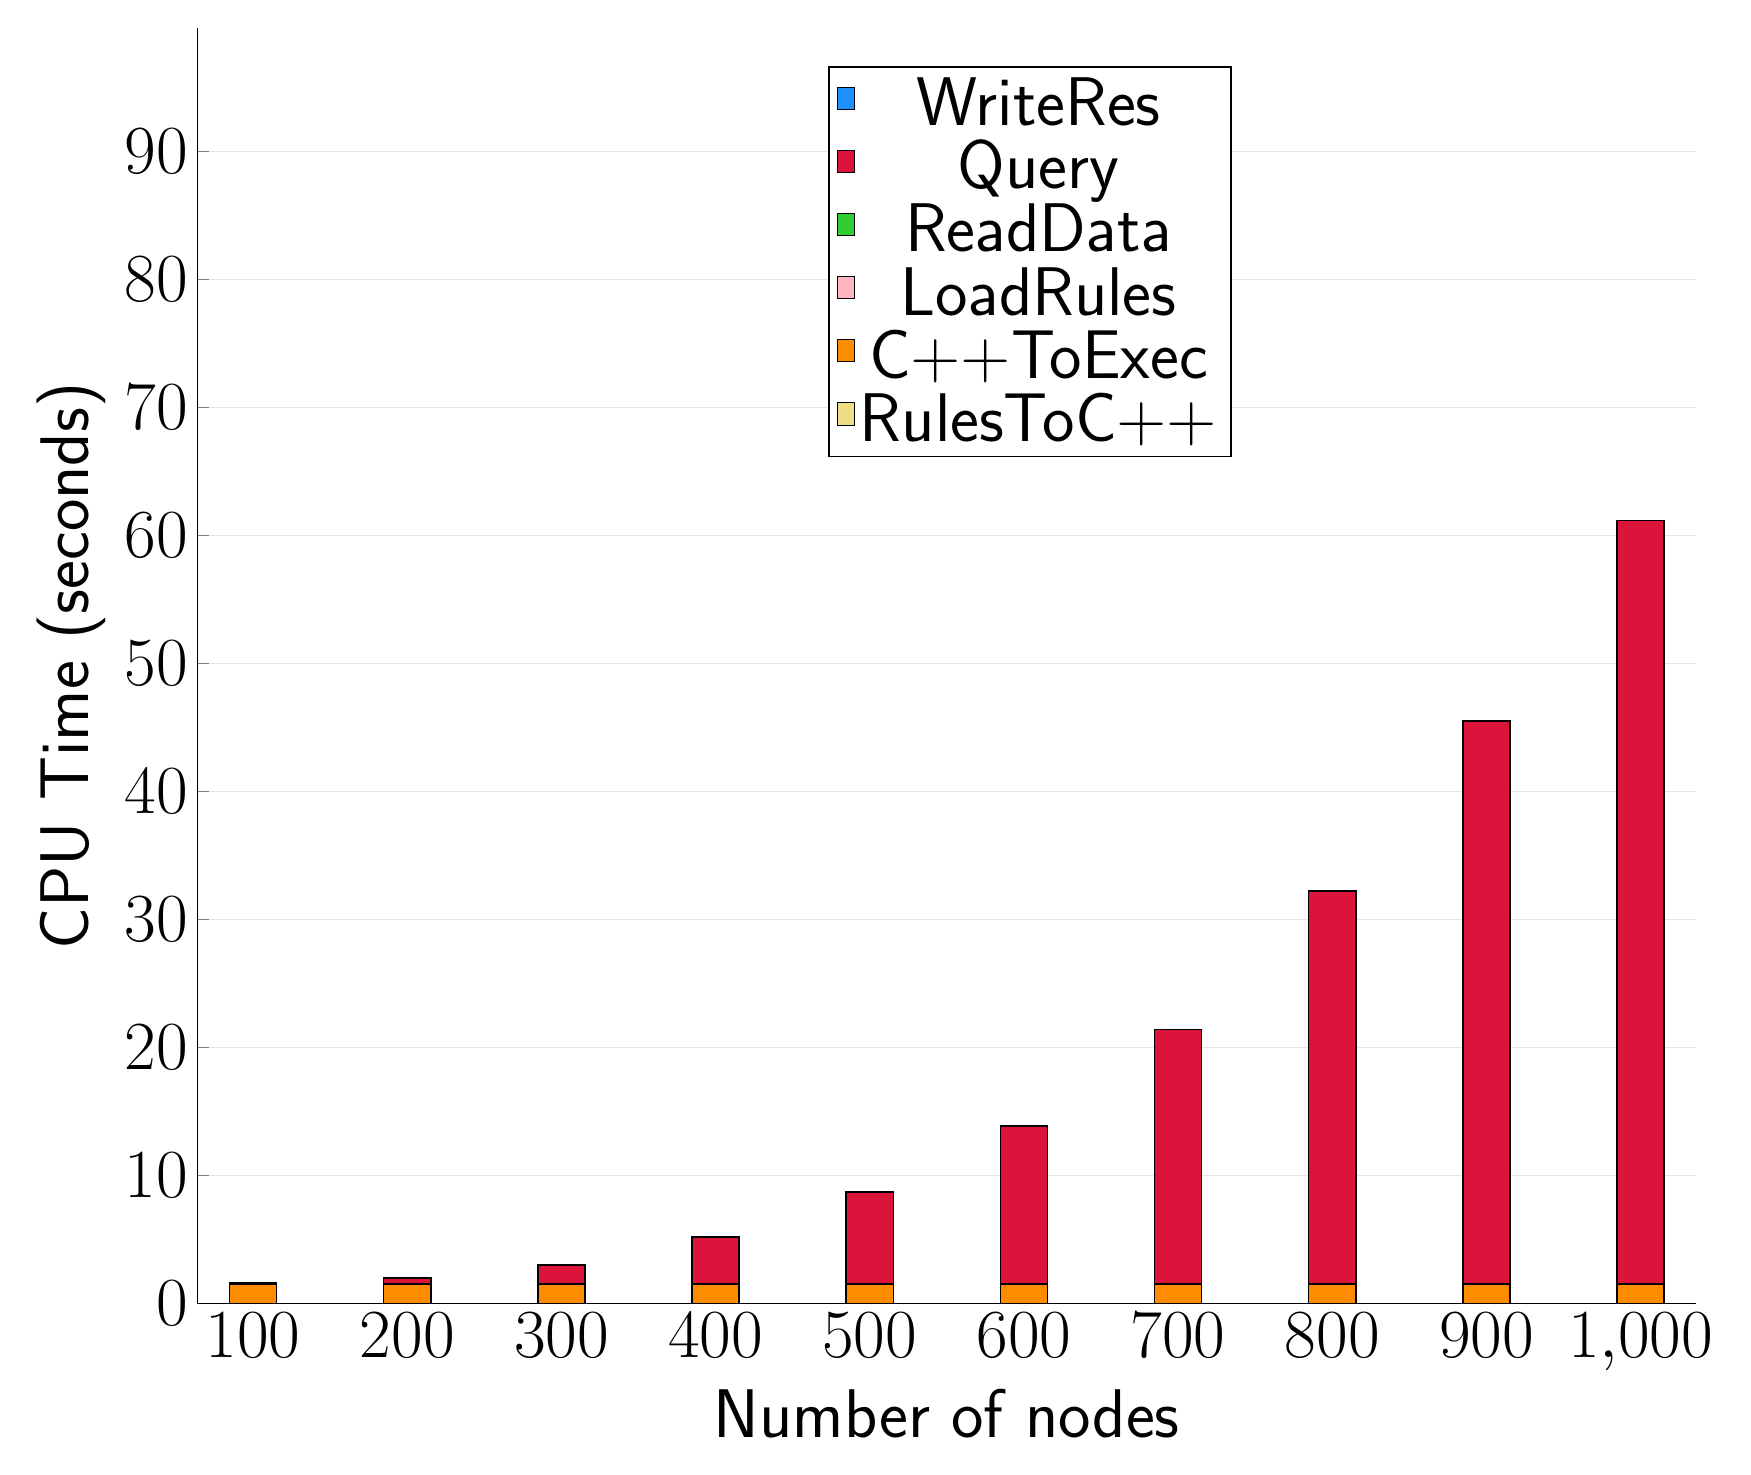
\begin{tikzpicture}
\begin{axis}[
   ybar stacked,
   width=1.7\textwidth,
   bar width=0.6cm,
   ymajorgrids, tick align=inside,
   major grid style={draw=gray!20},
   xtick=data,
   ymin=0, ymax=99.5987,
   axis x line*=bottom,
   axis y line*=left,
   enlarge x limits=0.04,
   legend style={
       at={(0.69, 0.97)},
       anchor=north east,
       legend columns=1,
       font=\Huge,
   },
   ylabel={CPU Time (seconds)},
   xlabel={Number of nodes},
   label style={font=\Huge},
   tick label style={font=\Huge},
]
\addlegendimage{fill=DodgerBlue, draw=black, line width=0.2pt}
\addlegendentry{WriteRes}
\addlegendimage{fill=Crimson, draw=black, line width=0.2pt}
\addlegendentry{Query}
\addlegendimage{fill=LimeGreen, draw=black, line width=0.2pt}
\addlegendentry{ReadData}
\addlegendimage{fill=LightPink, draw=black, line width=0.2pt}
\addlegendentry{LoadRules}
\addlegendimage{fill=DarkOrange, draw=black, line width=0.2pt}
\addlegendentry{C++ToExec}
\addlegendimage{fill=LightGoldenrod, draw=black, line width=0.2pt}
\addlegendentry{RulesToC++}
\addplot +[fill=LightGoldenrod, draw=black, line width=0.55pt] coordinates {
(100, 0.0020000000000000005)
(200, 0.004000000000000001)
(300, 0.008000000000000002)
(400, 0.008000000000000002)
(500, 0.006000000000000001)
(600, 0.008000000000000002)
(700, 0.008000000000000002)
(800, 0.0020000000000000005)
(900, 0.004000000000000001)
(1000, 0.006000000000000001)
};
\addplot +[fill=DarkOrange, draw=black, line width=0.55pt] coordinates {
(100, 1.532)
(200, 1.534)
(300, 1.54)
(400, 1.53)
(500, 1.5320000000000003)
(600, 1.5340000000000003)
(700, 1.53)
(800, 1.5240000000000002)
(900, 1.5320000000000003)
(1000, 1.53)
};
\addplot +[fill=LightPink, draw=black, line width=0.55pt] coordinates {
(100, 0.00015900000000000002)
(200, 0.000164)
(300, 0.000158)
(400, 0.0001702)
(500, 0.00016179999999999998)
(600, 0.000173)
(700, 0.0001762)
(800, 0.0001626)
(900, 0.0001874)
(1000, 0.00016659999999999998)
};
\addplot +[fill=LimeGreen, draw=black, line width=0.55pt] coordinates {
(100, 0.0008612)
(200, 0.001259)
(300, 0.0014878)
(400, 0.0020144)
(500, 0.0022572)
(600, 0.0028088)
(700, 0.0031690000000000004)
(800, 0.0033634000000000003)
(900, 0.0039884000000000005)
(1000, 0.0041022)
};
\addplot +[fill=Crimson, draw=black, line width=0.55pt] coordinates {
(100, 0.0763634)
(200, 0.46198259999999997)
(300, 1.4798680000000002)
(400, 3.6677999999999997)
(500, 7.185268000000001)
(600, 12.31096)
(700, 19.88186)
(800, 30.705720000000003)
(900, 43.95158)
(1000, 59.598699999999994)
};
\addplot +[fill=DodgerBlue, draw=black, line width=0.55pt] coordinates {
(100, 0.0002384)
(200, 0.00039)
(300, 0.0003356)
(400, 0.00040359999999999994)
(500, 0.000429)
(600, 0.0004364)
(700, 0.0004942)
(800, 0.00044280000000000003)
(900, 0.00043019999999999994)
(1000, 0.0005012)
};
\end{axis}
\end{tikzpicture}

\end{document}
